\subsection{Экспериментальная проверка принципа взаимности}

Принцип взаимности можно сформулировать следующим образом:

Если источник напряжение (единственный в цепи),
действуя в одной ветви линейной электрической цепи,
вызывает ток в другой ветви, то тот же источник после его
переноса во вторую ветвь вызовет в первой ветви такой же ток.

\begin{figure}[!h]
    \centering
    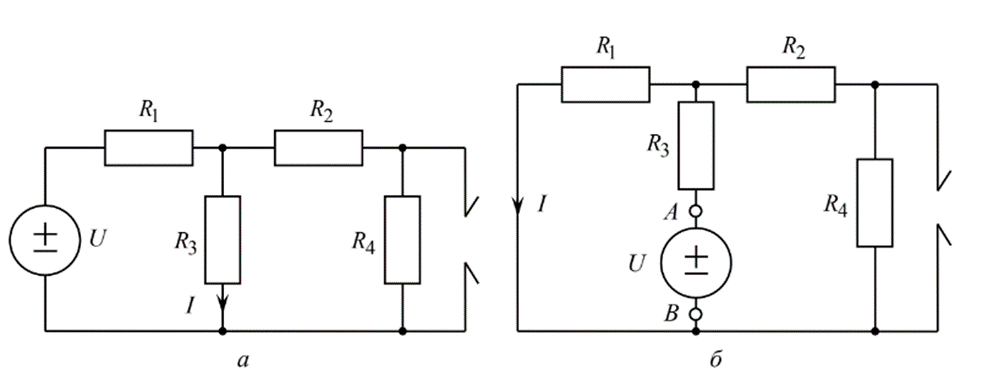
\includegraphics{reciprocity_1.png}
    \caption{Схема для проверки принципа взаимности}
\end{figure}

По результатам эксперимента $I_3=I_1^\prime$: $0,32\ \text{мА} = 0,32\ \text{мА}$.
Значит принцип подтверждается на практике.

